\documentclass[../SustainableHEP.tex]{subfiles}
\graphicspath{{\subfix{Sections/Figs/}}}
\begin{document}
\RaggedRight
\sloppy
\newpage

%%%%%%%%%%%%%%%%%%%%%%%%%%%%%%%%%%%%%%%%%%%%%%%%%%

\section{Research Infrastructure and Technology}
\label{sec:Technology}

%%%%%%%%%%%%%%%%%%%%%%%%%%%%%%%%%%%%%%%%%%%%%%%%%%

\begin{figure}
    
\includegraphics[width=\SDGsize]{Common/SDG_6_CleanWater.png}~%
    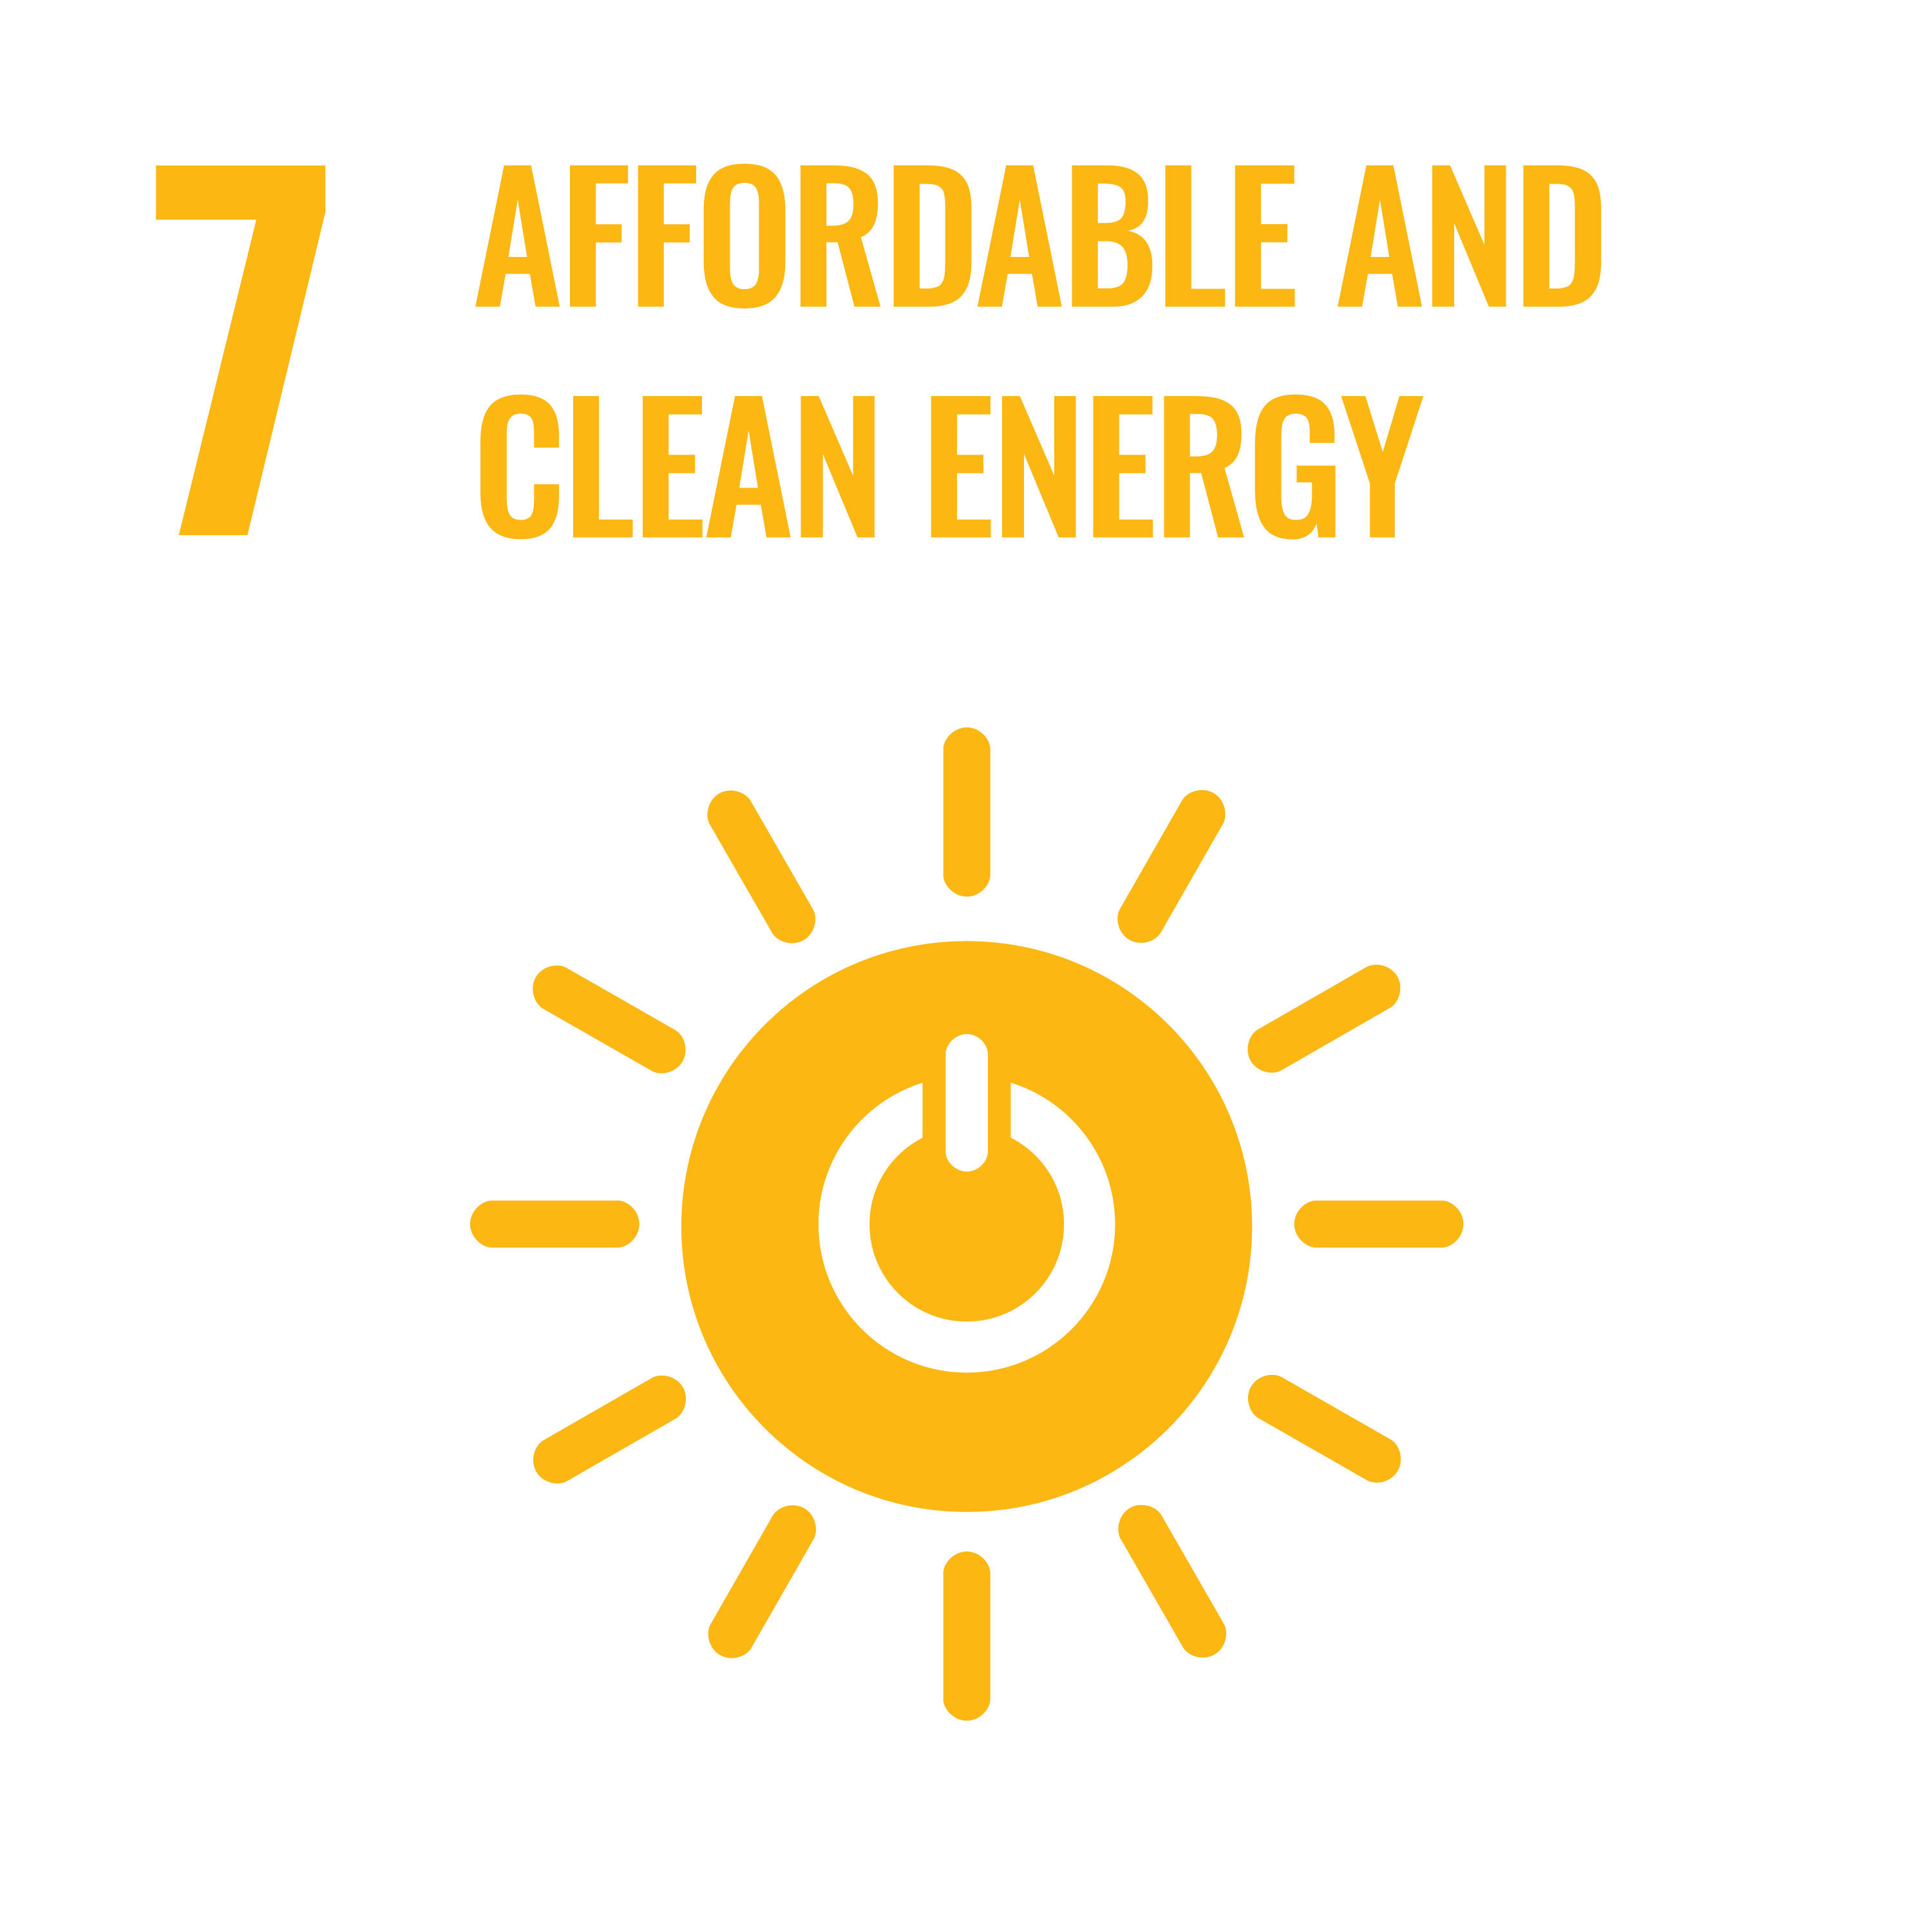
\includegraphics[width=\SDGsize]{Common/SDG_7_CleanEnergy.png}~%
    
\includegraphics[width=\SDGsize]{Common/SDG_9_IndustryInnovation.png}~%
    
\includegraphics[width=\SDGsize]{Common/SDG_11_SustainableCities.png}~%
    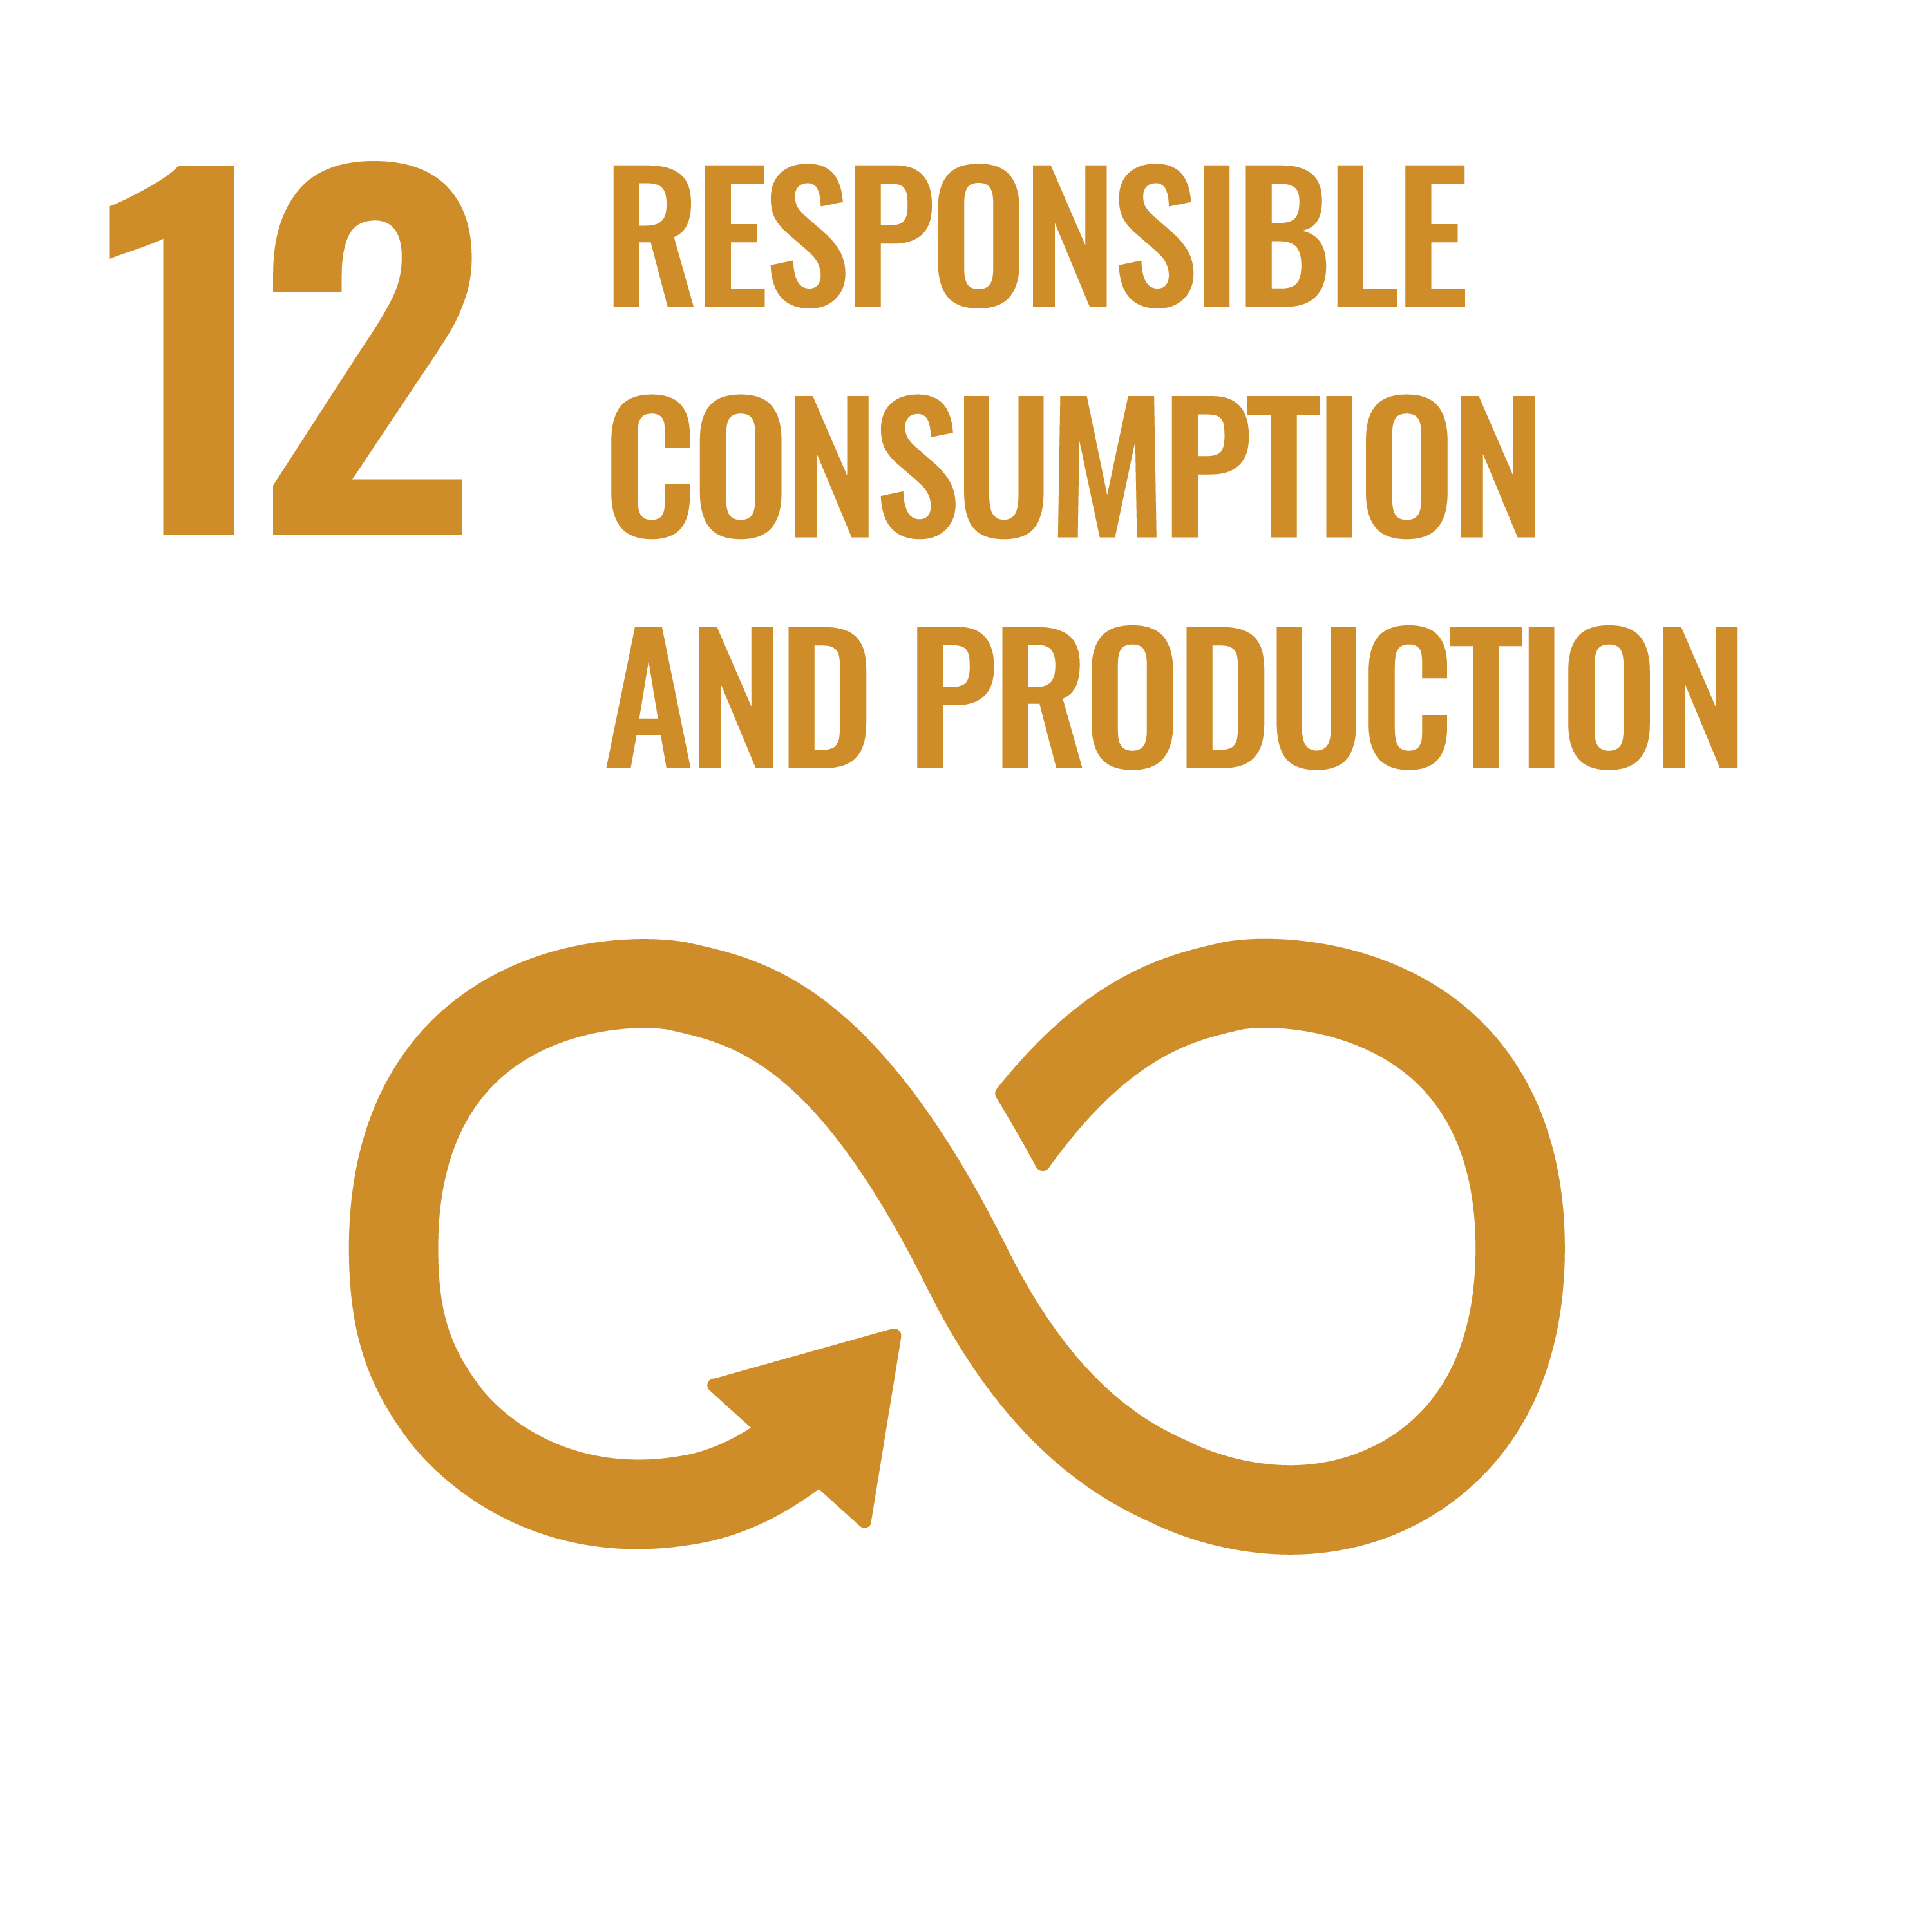
\includegraphics[width=\SDGsize]{Common/SDG_12_ResponsibleConsumption.png}~%
    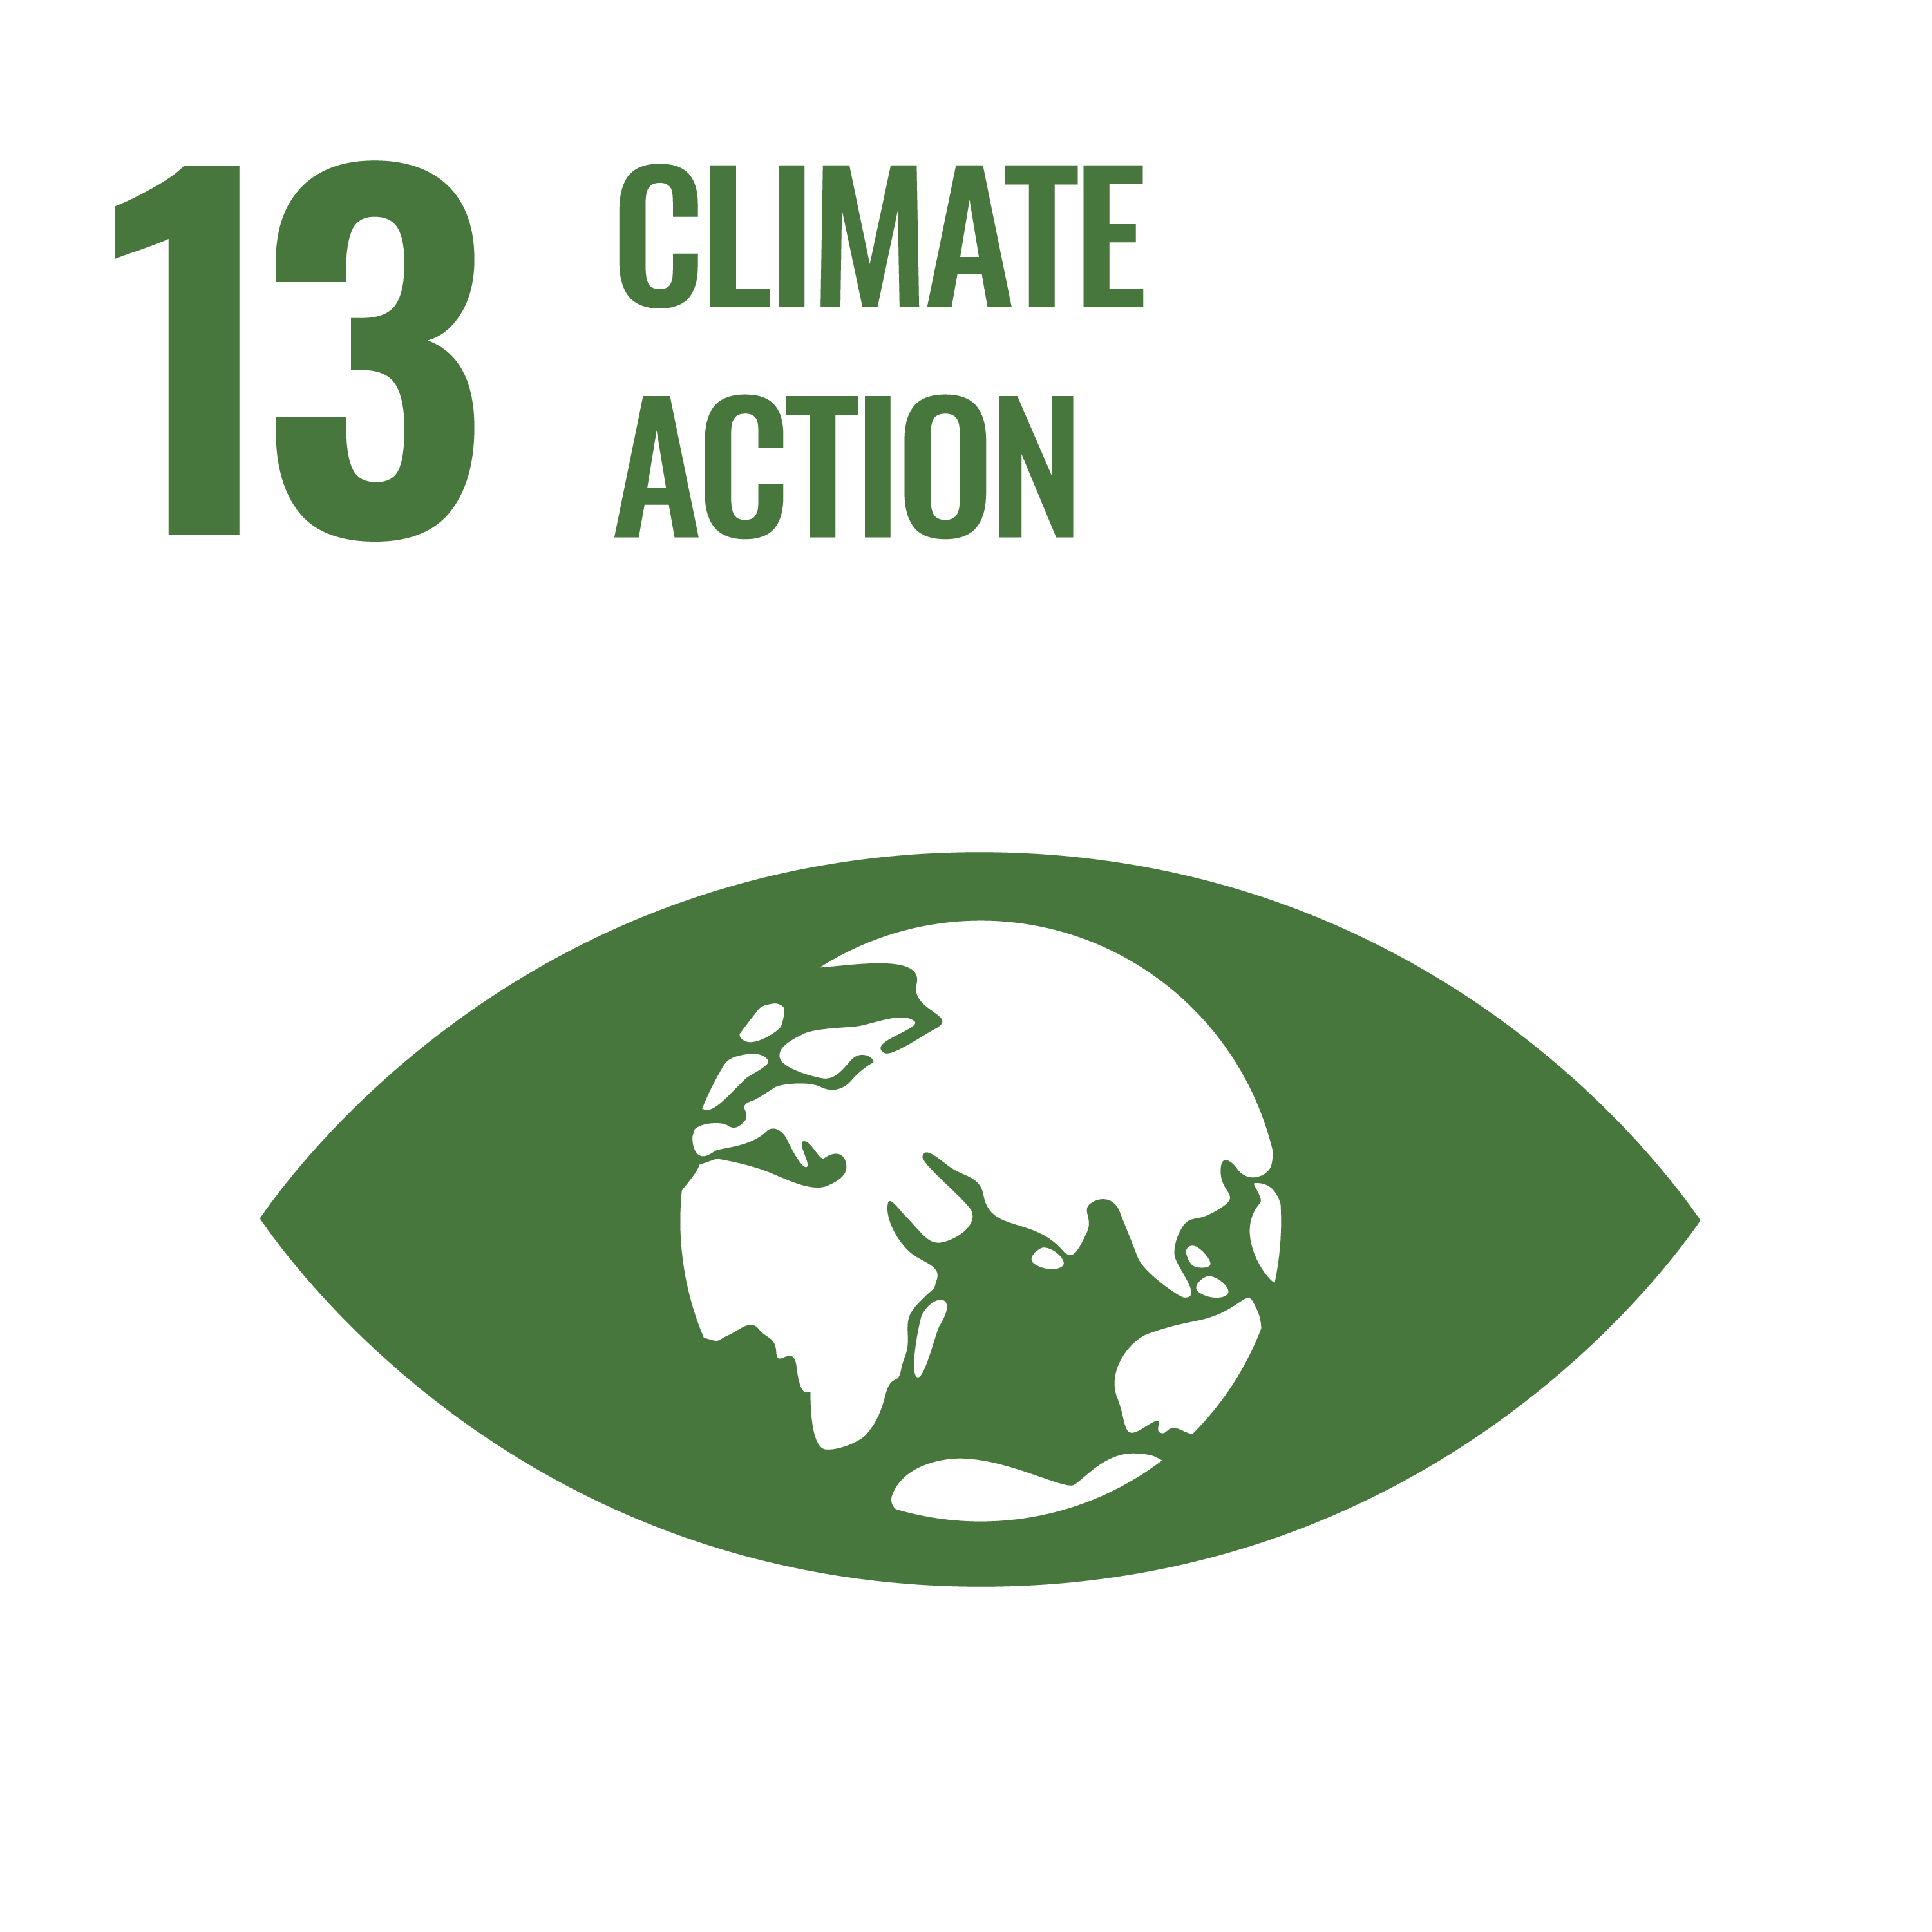
\includegraphics[width=\SDGsize]{Common/SDG_13_ClimateAction.png}~%
    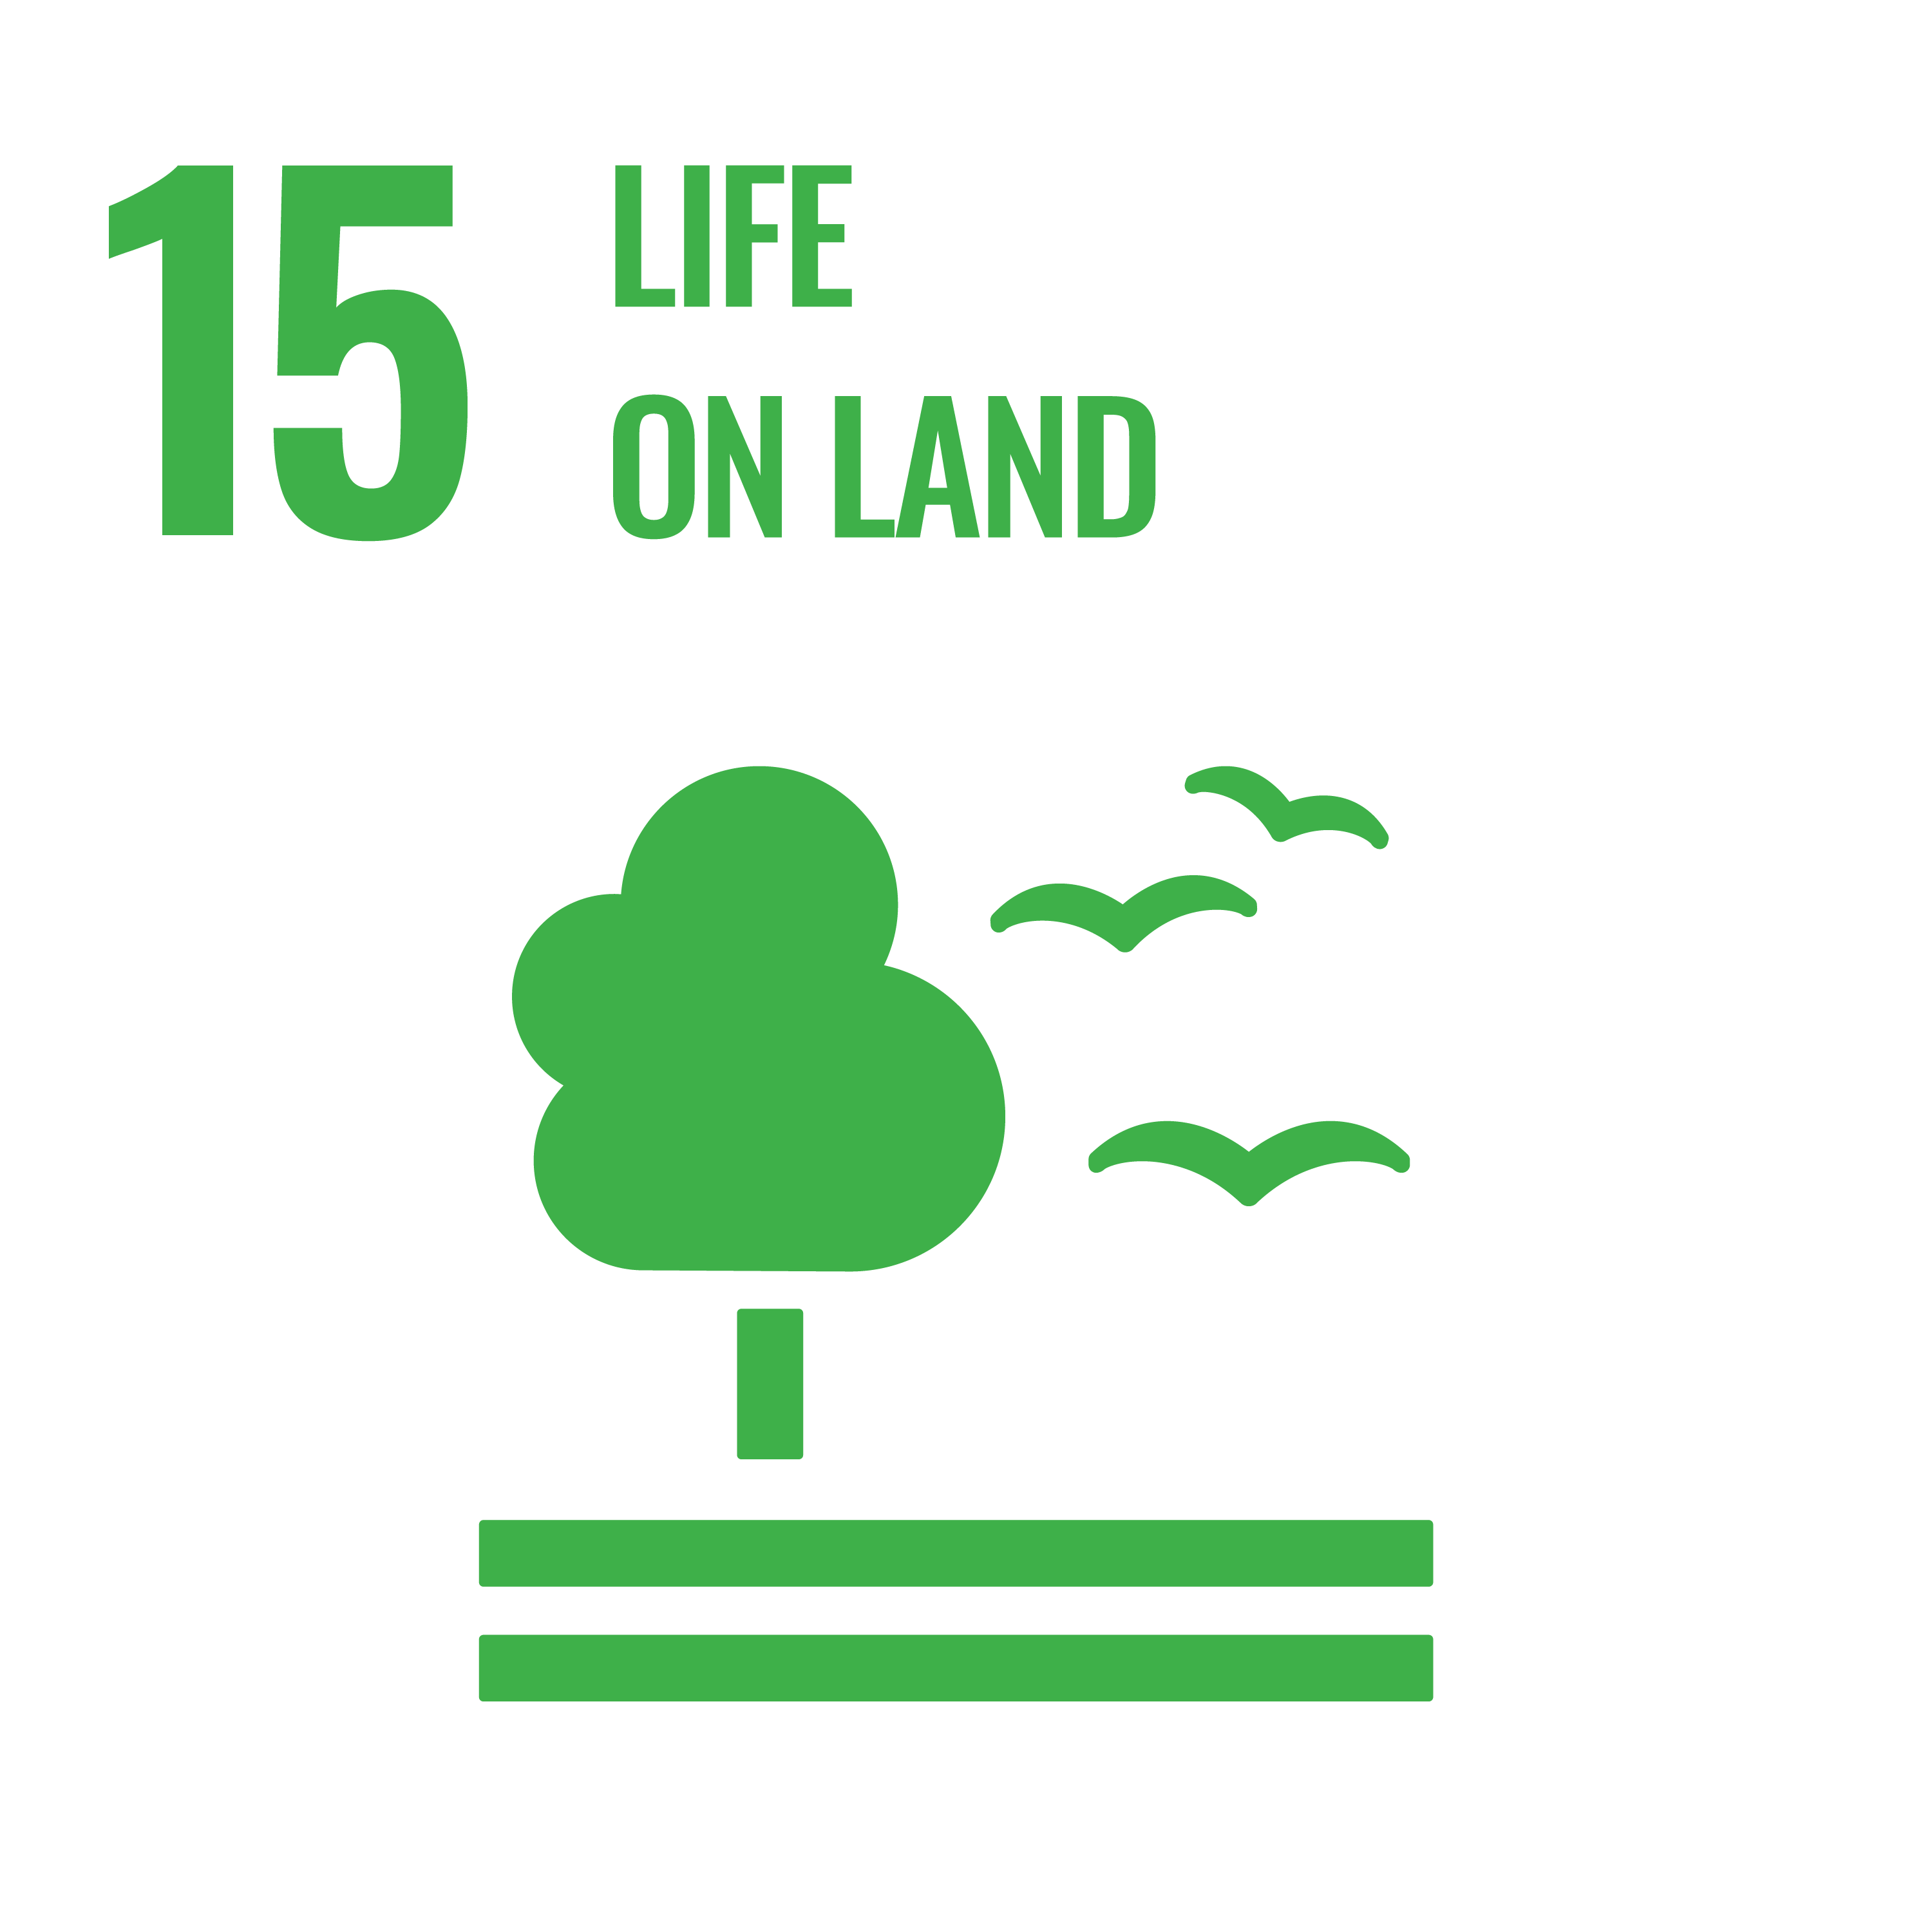
\includegraphics[width=\SDGsize]{Common/SDG_15_LifeOnLand.png}
\end{figure}

%%%%%%%%%%%%%%%%%%%%%%%%%%%%%%%%%%%%%%%%%%%%%%%%%%

\exSum

\noindent \acrshort{hecap} research areas rely on big science infrastructure. These particle accelerators, large-scale collider experiments, observatories and associated buildings infrastructure have a lifetime environmental impact from cradle to grave. This is recognised in Section 8, ``Sustainability considerations'', in the Accelerator R\&D Roadmap of the European Strategy for Particle Physics~\cite{EuropStrategyPP}. It divides the topic into three aspects:
\begin{itemize}
    \item Energy efficient technologies,
    \item Energy efficient accelerator concepts, and
    \item General sustainability aspects.
\end{itemize}
The first two focus on the biggest impact of accelerators:\ the energy consumption during their operation. One aspect focuses on the current technology and its energy efficiency, the other on the development of new accelerator concepts with smaller energy requirements. These topics are discussed in depth in other sections of the Strategy. The third aspect is more broadly defined and considers sustainability beyond energy~\cite{EuropStrategyPP}:
\begin{quotation}
    ``A carbon footprint analysis in the design phase of a new facility can help to optimise energy consumption for construction and operation. For cooling purposes accelerator facilities typically have significant water consumption. Cooling systems can be optimised to minimise the impact on the environment. For the construction of a facility environment-friendly materials should be identified and used preferably. The mining of certain materials, in particular rare earths, takes place in some countries under precarious conditions. It is desirable to introduce and comply with certification of the sources of such materials for industrial applications, including the construction of accelerators. A thoughtful life cycle management of components will minimise waste.''
\end{quotation}

In the case of astronomy research, Ref.~\cite{Kn_dlseder_2022} argues that emissions due to research infrastructure dominate the carbon footprint of an astronomer.

A number of initiatives have already been formed to consider the manifold technical challenges of improving the environmental sustainability of research infrastructure and associated technologies. Three examples are listed below, (for others see \sref{sec:other_initiatives} and references therein):
\begin{itemize}

    \item The International Committee for Future Accelerators (ICFA) has the specific panel ``Sustainable Accelerators and Colliders''~\cite{SustainableAcceleratorsICFA}.
    
    \item Every 2 years since 2011, the Energy for Sustainable Science at Research Infrastructures (ESSRI) workshop~\cite{ESSRI5} takes place.
    
    \item Innovation Fostering in Accelerator Science and Technology (\acrshort{ifast})~\cite{IFAST} is an EU-project in which the “WP 11 – Sustainable concepts and technologies” is aimed to increase sustainability. The current participating institutes are \acrshort{cern}, \acrshort{desy} in Germany, the European Spallation Source (ESS) in Sweden, the GSI in Germany, the Paul Scherrer Institut (PSI) in Switzerland, and the Science and Technology Facilities Council (\acrshort{stfc}) in the United Kingdom.

\end{itemize}
Environmental sustainability is also being considered by individual experiments, and \csref{case:LHCb} provides a summary of efforts by the \acrshort{lhcb} collaboration to assess and mitigate the environmental impact of both the experiment and work practices, more generally.

In this section, we consider the following aspects of environmental sustainability in research infrastructure: life cycle assessment (LCA), (carbon) accounting, and technological developments, particularly in the context of accelerator technologies and detector gases. While the discussions of technological developments provide concrete examples, the primary focus of this section is the need for critical life cycle analysis for all research infrastructure projects to assess and limit their environmental impacts. The impacts of mining and processing of materials is also considered in~\sref{subsec:Resources}, wherein complementary aspects of the LCA are also discussed.

\clearpage
\begin{reco2}{\currentname}
{
\begin{itemize}[leftmargin=6 mm]
\setlength{\itemsep}{\recskip}
\item Seek out new innovations and best practice.

\item Rethink how the impact of frequently-used equipment can be reduced, and reduce "over-design" by reassessing safety factors and other margins to reduce resource consumption.

\item Read section on resources and waste (Section~\ref{sec:Waste}).

\end{itemize}
}
{
\begin{itemize}[leftmargin=6 mm]
\setlength{\itemsep}{\recskip}
\item  Ensure that environmental sustainability is an essential consideration at all stages of projects, from initial proposal, design, review and approval, to assembly, commissioning, operation, maintenance, decommissioning and removal, using life cycle assessment and related tools.

\item Engage with industrial partners who exemplify best practice and sustainable approaches.

\item Appoint a dedicated sustainability officer to oversee project development, and institute regular meetings with a focus on environmental sustainability.

\end{itemize}
}
{
\begin{itemize}[leftmargin=6 mm]
\setlength{\itemsep}{\recskip}
\item Critically assess the environmental impact of materials, construction and the operational life cycle as an integral part of the design phase for all new infrastructure.

\item Provide training opportunities, required tools and technical support to assess and improve the environmental sustainability of project life cycles.

\item Recognise and reward innovations that minimise negative environmental impacts, regardless of revenue.

\item Promote knowledge exchange on sustainability initiatives between groups and institutions, including decision-makers, designers and operators of projects, setups and infrastructure.
\end{itemize}
}

\end{reco2}

%%%%%%%%%%%%%%%%%%%%%%%%%%%%%%%%%%%%%%%%%%%%%%%%%%

\subsection{Accounting and Reporting}


%\end{table}



The methodology of a life cycle assessment can be used to analyse the environmental impact of resources used to build, run and decommission an accelerator, observatory or experiment, see Section~\ref{sec:sustainablesourcing} for further details. Such assessments have already been undertaken by a number of facilities, including:
\begin{itemize}
    \item The European Southern Observatory (ESO)~\cite{ESO}.
    \item The Giant Radio Array for Neutrino Detection (GRAND) Project, a multi-decade astrophysics experiment~\cite{Aujoux_2021} --- This led to a full issue of the Nature Astronomy Journal on climate change~\cite{NatureClimateIssue}.
    \item The Relativistic Ultrafast Electron Diffraction and Imaging (RUEDI) facility at STFC Daresbury Laboratory ~\cite{Shepard}.
    \item The Compact Linear Collider (\acrshort{clic}) is planning to conduct an assessment ~\cite{privateBList}.
    \item The ISIS-II project, the next generation of the ISIS neutron and muon source, is planning to conduct life cycle analyses for the project and various design options ~\cite{ISISII}.
\end{itemize}

There is currently limited availability of data on estimated emissions and resources consumption for basic research infrastructure, and, where it is available, its presentation is not standardised. This makes overall assessments of sustainability and comparisons of individual technologies challenging. Implementation of effective life cycle assessment across the \ACR community could provide the impetus for standardised reporting that will provide the data needed for ongoing assessment of current and future technologies and research infrastructure projects, such as any future collider concept (see \csref{case:FutureColliders}).

See \bpref{bp:SiWafer} for a summary of life cycle assessment for a silicon wafer used in particle detectors, summarised from the ProBas library for life cycle assessment~\cite{ProBasSi}.

 The labos1point5 working group has proposed a standardised carbon accounting procedure and associated assessment tool for research laboratories. This programme is described in detail in \bpref{BP:l1p5}.

\begin{bestpractice}
[Life cycle assessment for a silicon wafer\label{bp:SiWafer}]{Life cycle data for a silicon wafer}%
%An example of an input material in the life-cycle assessment, relevant to particle detectors, are silicon wafers. 
The ecological impacts of a  1 ${\rm cm}^2$ silicon wafer (thickness 775 $\mu$m, diameter 300 mm, weight 0.128 kg) as identified in 2000, are summarised in Table~\ref{tab:InputOutputEmissions}~\cite{ProBasSi}.
\\
\bigskip
% Two tables in one
{\ra{1.01}
%\begin{table}
\centering
\captionsetup{type=table}
\resizebox{\textwidth}{!}{
\begin{tabular}{m{0.3\textwidth}m{0.2\textwidth}m{0.3\textwidth}m{0.2\textwidth}}

\toprule
Inputs&
Quantity&
Outputs&
Quantity\\
\midrule
Hydrogen chloride HCl (hydrochloric acid)&
0.00675 kg&
Co-products: Si in other co-products& 0.000286 kg\\
\midrule
Graphite (as electrode material)& 0.000163 kg & Co-products: Silicon tetrachloride & 0.00415 kg
\\
\midrule
Wood chips&
0.00183 kg & 
Co-products: Si residues for solar cells&
65.2 $\times10^{-6}$\\
\midrule
Petroleum coke& 0.000597 kg &
Polished silicon wafer&
1 cm$^2$\\
\midrule
Quartz&
0.00486 kg &
&
\\
\midrule
Electricity&
0.385 kWh&
& \\
\midrule
Dry wood & 0.00398 kg & &\\
\bottomrule
%\\
%\rule
% empty line 
%&
\\
\toprule
Air emissions&
Quantity&
Discharge to Water&
Quantity\\
\midrule
CH${}_4$&
68.8$\times$10$^{-6}$ kg&
Metal chlorides&
0.000787 kg\\
\midrule
CO&
0.000167 kg&
& 
\\
\midrule
CO${}_2$&
0.00833 kg&
Waste&
Quantity\\
\midrule
Ethane&
29$\times$10$^{-6}$ kg&
SiO${}_2$&
16.3$\times$10$^{-6}$ kg\\
\midrule
H${}_2$O&
0.00188 kg&
&
\\
\midrule
Methanol&
85.1$\times$10$^{-6}$ kg&
&
\\
\midrule
NOx&
13.8$\times$10$^{-6}$ kg&
&
\\
\midrule
Particulate matter&
0.000201 kg&
&
\\
\midrule
SO${}_2$&
34.4$\times$10$^{-6}$ kg&
&
\\
\midrule
Hydrogen&
0.000125 kg&
&
\\
\bottomrule
\end{tabular}
}
\caption[Inputs, outputs and emissions of silicon wafer production]{Inputs, outputs and emissions of silicon wafer production~\cite{ProBasSi}.}
\label{tab:InputOutputEmissions}
}

\end{bestpractice}
%%%%%


%\subsection{Accounting and Reporting}



%The methodology of life-cycle assessment is well established, and it can be used to estimate the impact and sustainability of \ACR-specific research technology. 


\begin{casestudy}[\label{case:FutureColliders}Sustainability of Future Colliders]{Sustainability of Future Colliders}%
\noindent The future of \acrshort{hep} includes decisions on Future Collider Facilities to be built. \fref{fig:powerCollider} compares the energy needs of Future electron-positron (e$^+$e$^-$) Colliders. The projected grid power during operation is given, including for the laboratory, computer center and detector.

\begin{figure}
    \captionsetup{type=figure}
    {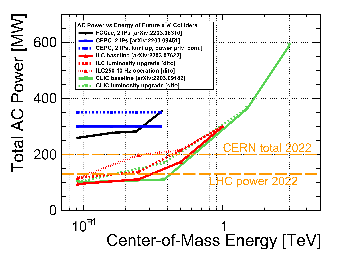
\includegraphics[width=.8\textwidth]{Technology/modified_power_vs_logE_withLHCandCERN.png}}
    \caption[Site power required for proposed $e^+e^-$ colliders]{Site power required for proposed electron-positron ($e^+e^-$) collider projects at different center-of-mass energies, compared to the power consumption of CERN and LHC in 2022~\cite{privateJList}. }\label{fig:powerCollider}
\end{figure}

The environmental sustainability of future facilities will become an increasingly important and heavily scrutinised factor in the decision making process about which, if any, facility should be built. The life cycle assessment for such facilities is extremely complex, and must cover not only the accelerator and the detectors, but also the civil engineering, such as tunnels and caverns, buildings infrastructure, and computing needs. The impact of construction, then deconstruction (except for the tunnel) and disposal (including activated materials, which may constitute a radiation hazard) after a few years is not negligible.

The evaluation of the \CdO\ footprint due to the electricity consumption of a future collider is particularly challenging, since any estimate relies heavily on assumptions about future electricity mix. A conservative estimate might be given based on the current \CdO\ footprint for electrical energy, under the assumption that the grid will be decarbonised --- indeed it has to be to meet the world's climate goals --- by the time any future collider is commissioned. However, there is the opportunity to adapt to potential sources of renewable energy (see also \sref{sec:Energy}) in the design stages, and to go beyond arguments of ``electrical effectiveness'' based on scientific benchmarks, such as kWh/Higgs or kWh/luminosity compared to the required connected power.
\end{casestudy}

\begin{bestpractice}
[Standardised accounting
of the carbon footprint of French research 
institutions: labos1point5 \label{BP:l1p5}]{Carbon footprint accounting with the Labos1point5 tool}%
\noindent \emph{Laboratoires de recherche}, loosely translated as research labs,
are the entities around which most of French research is organised.
They enjoy a relevant degree of autonomy, including 
aspects such as scientific goals and experimental designs. 
Access to research facilities, as well as 
a fraction of the annual budget is also managed at the lab scale.
Hence, this makes it a relevant scale to tackle the question 
of the carbon footprint of academic research. 

This has motivated the creation of the \emph{labos1point5} 
working group (\emph{Groupement De Recherche}, GDR),\footnote{``1point5''
refers to the warming limit of the Paris accord}
gathering an interdisciplinary team of engineers and researchers from various research fields in France. 
One of the main outputs of this collaboration is the \emph{GES 1point5},\footnote{``GES''
is the French acronym for greenhouse gases.} a
standardised online tool for the accounting of the carbon 
footprint of French research labs. What follows is a brief
summary of the latter. We refer to Ref.~\cite{labos1p5}
for a publication describing it. Further information 
can be found on the website of the labos1point5 collaboration~\cite{labos1p5web}. The tool itself is available at \cite{ges1p5}, 
while the open source code is hosted at \cite{ges1p5git}.
The GDR labos1point5 is also active in helping labs in their
transition to a lower footprint, in developing new ways of 
teaching climate and ecological aspects to students, as well
as of communicating to the general public. Finally,
there are  teams dedicated to the reflection on the role
of science in the climate crisis, and on fostering collaboration 
between arts and science in this context.

As explained in Ref.~\cite{labos1p5}, one of the main motivations for the 
creation of the GES 1point5 tool was the difficulty in aggregating or comparing the results of 
the many existing studies in the literature on the carbon footprint of academic research.
This difficulty was caused by the sensitivity of the footprint to the applied 
methodology, which made comparisons extremely challenging, since discrepancies in results
could not be disentangled from methodological differences. 
The creation of the GES 1point5 was then intended to provide 
a tool specifically designed to estimate the carbon footprint of research with a transparent
and accessible methodology and a database of carbon footprints assessed with the same
methodology to enable a robust comparison of research carbon footprints across institutions,
contexts or disciplines.

More specifically, GES 1point5 allows research labs to
estimate their yearly emissions --- as of February 15, 2023,
628 laboratories have compiled 1,140 yearly carbon footprint 
determinations \cite{labos1p5web}.
Currently, GES 1point5 can estimate \acrshort{ghg} emissions 
due to the energy consumption and refrigerant gases of the laboratories' buildings, 
those attributed to the purchase of their digital devices, and to computing, 
commuting and professional travel, as well as the associated uncertainties.
A module estimating emissions from consumables purchases has recently been added.
In all cases, the estimation is based upon its established
standardised methodology, and the database of emission factors, and turns out 
to be relatively straightforward for the end user.\footnote{In the case
of professional travel, a feature has been added to the internal management software
of the French National Centre for Scientific Research (CNRS) that can output the travel data --- origin, destination, means of transportation, etc.~---
for a given year in a ready-for-GES 1point5 format,
sparing the end user tedious data entry/conversion.} To give an example, 
commuting emissions are estimated by gathering data through an anonymised survey
sent to staff members, which can be answered in less than five minutes.
For each specified commute (up to two different ones per week can be entered)
GES, 1point5 multiplies the distance traveled via each means of transportation by
the specific emission factor from its database. These are collected in \fref{fig:emiMobility} in \sref{sec:Travel}.
The underlying routines are available at \cite{1p5commute} for everyone to test their 
commutes; similarly, those used in the determination of professional travel emissions are 
available at \cite{1p5travel} and those for purchases at 
\cite{1p5purchases}.

Once the emissions have been estimated, GES 1point5 presents the results 
through its graphical interface, highlighting the main drivers of the carbon footprint. 
Finally, emissions reduction actions that may be undertaken after the evaluation of the 
footprint can be evaluated in the subsequent years, thanks to the reliance
on a standardised protocol. The latter also allows the aforementioned 
aggregation and comparison of GES 1point5-based carbon footprints.

As stated in Ref.~\cite{labos1p5}, while some aspects of GES 1point5 are specific 
to the context of French research, the tool  may be reused in research centers elsewhere, provided
the necessary adjustments --- e.g., carbon intensity of the grid --- are taken. 
A French- and an English-language version of GES 1point5 are built into the current version to ease deployment in any country; contacts with several institutions outside France 
have been established.
\end{bestpractice}

%%%%%%%%%%%%%%%%%%%%%%%%%%%%%%%%%%%%%%%%%%%%%%%%%%

\subsection{Technological Improvements}

There are ongoing efforts across the \ACR community to reduce the environmental impacts of the technologies implied in research facilities. Two examples in the case of acccelerator technologies are provided in Best Practice~\ref{BP:EnergyRecoveryAccelerator} and Case Study~\ref{case:wakefield}, namely energy-recovery accelerators and plasma wakefiled acceleration technologies. Further details of efforts by the \acrshort{lhcb} collaboration are included in \csref{case:LHCb}. A detailed discussion of the impact of detector gases is provided in the following subsection.

\begin{bestpractice}[\label{BP:EnergyRecoveryAccelerator}Realization of a multi-turn energy-recovery accelerator]{Multi-turn energy-recovery accelerator}%
\noindent The operation of particle accelerator facilities is inherently resource-intensive, and thus poses a challenge to sustainability. In line with acknowledging our responsibility for sustainable usage of energy resources, the development, establishment, and demonstration of a scalable multi-turn Energy Recovery Linac (ERL) with efficient energy recycling was implemented at the S-DALINAC accelerator at TU Darmstadt, Germany~\cite{Arnold:2020snn}. An efficient energy-recycling in multi-turn operation with a saving of up to 87 \% of the beam power-consumption in the main LINAC has been recently demonstrated. This result, together with further developments on multi-turn ERLs is a promising basis for future high-power beams that truly support sustainability aspects. (Other examples include ER@CEBAF in the USA~\cite{Meot:2018yoo}; MESA ERL in Germany~\cite{MESA}; International PERLE Collaboration~\cite{PERLE, PERLECDR}; CBETA, the Cornell-BNL ERL Test Accelerator~\cite{CBETACDR}; for an overview, see Refs.~\cite{Klein:2022lgx, Hutton:2022kac}).
\end{bestpractice}

\begin{casestudy}[Sustainability of plasma wakefield acceleration technology for future accelerators\label{case:wakefield}\\{\noindent\footnotesize{Contribution by Nikola Crnkovi\'{c}}}]{Plasma wakefield for future accelerators}%
\noindent  A promising technology which would reduce both the material and energy cost of accelerating particles, and hence improve its environmental sustainability, is wakefield acceleration~\cite{wakefield1}.  These use laser pulses (in the case of laser wakefield accelerators), or particle beam bunches (for plasma wakefield accelerators, PWFAs) as the driver to accelerate plasma electrons, creating ion cavities.  This creates an electric field that pulls electrons back to their original positions, which they overshoot, creating waves in the plasma, known as the wakefield.  These plasma waves can accelerate electrons by transferring energy from the drive beam to electrons by putting electrons just behind the drive beam.  Wakefield technology routinely gives acceleration gains of $10$--$100$ GeV/m \cite{wakefield1}, thus resulting in a significant reduction of the resources required (materials, energy) to build particle accelerators.  For example, accelerating electrons to 1 TeV of energy using PWFA would require, \eg only a 21 km-long particle accelerator, while CLIC technology needs 52 km~\cite{wakefield2}.  Furthermore, there are indications that PWFA is more power efficient at high energies than conventional accelerator technology~\cite{wakefield2}.
\end{casestudy}

\subsubsection{Gases}

Significant quantities of GHGs are used for particle detection technologies and cooling systems across \ACR. As such they are used as a resource, but can escape the detector volume into the atmosphere and turn into potentially dangerous waste gases. Table~\ref{tab:GasImpact} lists a number of GHGs, their chemical formulae, atmospheric lifetimes and global warming potentials (\acrshort{gwp}). All of these gases are used either for cooling purpose or as active ingredients in gaseous detector systems, where they are often added to noble gases to improve detector properties, such as drift charge velocities or diffusion coefficients~\cite{Sauli:2014cyf}.
    

{\centering
\ra{1.1}
\captionsetup{type=table}
\begin{tabular}{@{}lllc@{}}\toprule
Name& Chemical\,\,\; & 
Lifetime\,\,

& Global warming potential (GWP) \\ 
&  Formula& 

[years]
& [100-yr time horizon]\\ 
\midrule
Carbon dioxide &	CO$_2$ & -- & 1 \\
Dimethylether& CH$_3$OCH$_3$ & 0.015 & 1 \\ 
Methane & CH$_4$& 12& 25\\
Sulphur hexafluoride& SF$_6$ & 3,200 & 22,800\\
\midrule
\multicolumn{4}{c}{Hydrofluorocarbons (HFCs)}\\
\midrule
HFC-23 & CHF$_3$ &  270 & 14,800\\
HFC-134a & C$_2$H$_2$F$_4$ & 14 & 1,430\\
\midrule
\multicolumn{4}{c}{Perfluorocarbons (PFCs)}\\
\midrule
PFC-14 & CF$_4$ & 50,000 & 7,390 \\
PFC-116& C$_2$F$_6$ & 10,000  & 12,200\\
PFC-218&C$_3$F$_8$ & 2,600 & 8,830 \\
PFC-3-1-10 &C$_4$F$_{10}$ & 2,600 &8,860\\
PFC-5-1-14 &C$_6$F$_{14}$ & 3,200 & 9,300\\
\bottomrule
\end{tabular}
\caption[Warming potential of selected GHGs]{Environmental impact associated with GHGs, from Ref.~\cite{IPCC17technical}, which also forms the source for the calculations in the CERN environmental report and the EU regulations described in~Ref.~\cite{EUFgasregulation}.}\label{tab:GasImpact}
}

Whilst gases are used in a variety of detectors, such as time projection chambers, ring-imaging Cherenkov detectors or multi-wire proportional chambers, the main offenders in ecological terms are the detectors used in the muon systems of the LHC experiments, specifically resistive plate chambers (RPCs). This is due to their large areas of around 7,000 m$^2$ in total for both the CMS and ATLAS muon systems, and the gas mixtures used to cope with the large event rates at the LHC, which often feature HFC-134a as main component. 

As shown in Figure~\ref{fig:Intro-ComparativeEmissions}, Scope 1 direct emissions made up about 25\% of CERN's carbon footprint in 2019. During the LHC Run 2 in 2018, it was about a factor of two larger.  92\% of these Scope 1 emissions are related to the activities of the large LHC experiments~\cite{Environment:2737239,envrep2020}. CERN and the LHC experiments are actively working on reducing this impact by continuously repairing gas leaks that are one of the main reasons for the large amount of waste gas. In addition, CERN has tested an HFC-134a recuperation plant showing an efficiency of close to 85\%, which is to be installed in the detectors to reduce the environmental impact~\cite{envrep2020}, and is actively researching alternative gas mixtures~\cite{Mandelli:2022qjc}. Future detector projects still plan to use RPCs (DUNE covering an area of about 860 m$^2$~\cite{DUNE:2016rla} and SHIP with about 100 m$^2$~\cite{SHiP:2021nfo}) but are testing their prototypes also with alternative gas mixtures~\cite{Albanese_2023}.  

The gases responsible for about 80\% of CERN's Scope 1 direct annual GHG emissions are sulphur hexafluoride (SF$_6$), hydrofluorocarbons (HFC) and perfluorocarbons (PFC) in particle detection, and HFCs and PFCs for detector cooling. To put the emissions into context, CERN's SF$_6$ emissions are about 5\% of Switzerland's, and of the same size as those of Luxembourg or Latvia \cite{SF6data}. All of these so-called F-gases have EU supply restrictions imposed on them since 2015~\cite{EUFgasregulation}, effectively phasing out their usage. A 2022 regulation proposal aims to extend EU regulations, \eg to reduce HFC usage down to 98\% by 2050 compared to 2015 levels. An additional significant factor in this proposal is the removal of certain sector exemptions for HFC usage, such as research. All of this could significantly impact the availability and cost of F-gases in the future and therefore affect the \ACR\ community, which should be reflected in the plans for ongoing and future experiments. Even independent of these EU regulations, the \ACR\ community should work with highest priority on abolishing GHGs in existing and future detectors. Ideally this would consist of replacing them with non-GHGs, or gases with low GWP,  or gasless detector technology.

In some scenarios, low-GWP gases used as replacements for industrial applications are not suitable for detector applications and, as such, studies for alternative gases are currently ongoing. The difficulty in finding replacement gases originates from having to satisfy several factors: safety (non-flammable and low toxicity) and environmental impact (minimising GWP), while maintaining their detector performance (including preventing the ageing of the detectors, ensuring good quenching\footnote{Quenching is the prevention of secondary electron avalanche (and thus signals) caused by, \eg photon emissions of the positive ions in the gas when recombining with electrons. As the positive ions travel more slowly through the gas detectors, these secondary signals happen after the primary signal from the electrons are registered and cause significant dead-times, when the detector is not responsive to new signals.} and being radiation-hard)~\cite{Bloom:2022gux}.

Current gas mixture alternatives for particle detection are centred around tetrafluoropropene (chemical formula C$_3$H$_2$F$_4$ and industrially referred to as HFO-1234ze/R-1234ze). The mixture has zero ozone-depletion potential and a global warming potential below 1, over a span of 100 years. Simulations of RPCs that operate with various gas mixtures, which include R-1234ze, have shown promising results, although further studies are still required~\cite{Fan:2022azj_ref3,Proto:2021taf_ref4}.

Long term, it is crucial to design future detector systems with gas GWP in mind. Consequently, it is essential that current state-of-the-art and future detectors are compatible with this and, if not, R\&D is aimed at reducing the GHG emissions of such systems.

\begin{casestudy}[LHCb and sustainability\label{case:LHCb}\\\noindent {\footnotesize Edited from Framework TDR for the LHCb Upgrade II~\cite{LHCbU2FTDR}: Opportunities in flavour physics, and beyond, in the HL-LHC era, edited extracts from the U2 FDTR chapter on environmental impacts of the project, as contributed by Chris Parkes.}]{LHCb and sustainability}%
\noindent In a world with increasing demand on limited resources and undergoing climate change, the LHCb collaboration feels a responsibility to consider energy consumption, sustainability and efficiency when discussing our scientific proposals. To this end the Framework Technical Design Report of the next-generation LHCb Upgrade II experiment~\cite{LHCbU2FTDR} has included a dedicated chapter on these considerations analysing the current Upgrade I system and indicating directions for future investigation. This section reports some of the main elements.  

The 2020 update of the European Strategy for Particle Physics~\cite{EuropeanStrategy2020} reports: ``The environmental impact of particle physics activities should continue to be carefully studied and minimised. A detailed plan for the minimisation of environmental impact and for the saving and re-use of energy should be part of the approval process for any major project. Alternatives to travel should be explored and encouraged.'' 
As one of the major experimental infrastructures operating at the LHC,  our environmental protection strategy should be made in coordination with CERN guidelines, as described in the first CERN environment report~\cite{envrep2020}.

CERN has a formal objective to reduce direct emissions (``Scope 1'') by $28\%$ by the end of 2024. These are dominated by the activities of the LHC experiments, and in particular by the use of fluorinated gases for particle detection and detector cooling purposes, as shown in \fref{fig:cern_co2}. These emissions have to be carefully considered in the operation of the Upgrade I detector and in the design of its future upgrade. Other relevant aspects of the environmental impact of our project are the power consumption of the experimental infrastructure (indirect emissions, ``Scope 2''), the impact of digital technologies, and travel of the members of the collaboration. \fref{fig:lhcb_co2} shows the relative contribution of each of these sources to the CO$_2$ equivalent footprint of the experiment operations expected during Run 3. %}

\begin{figure}
    \captionsetup{type=figure}
    {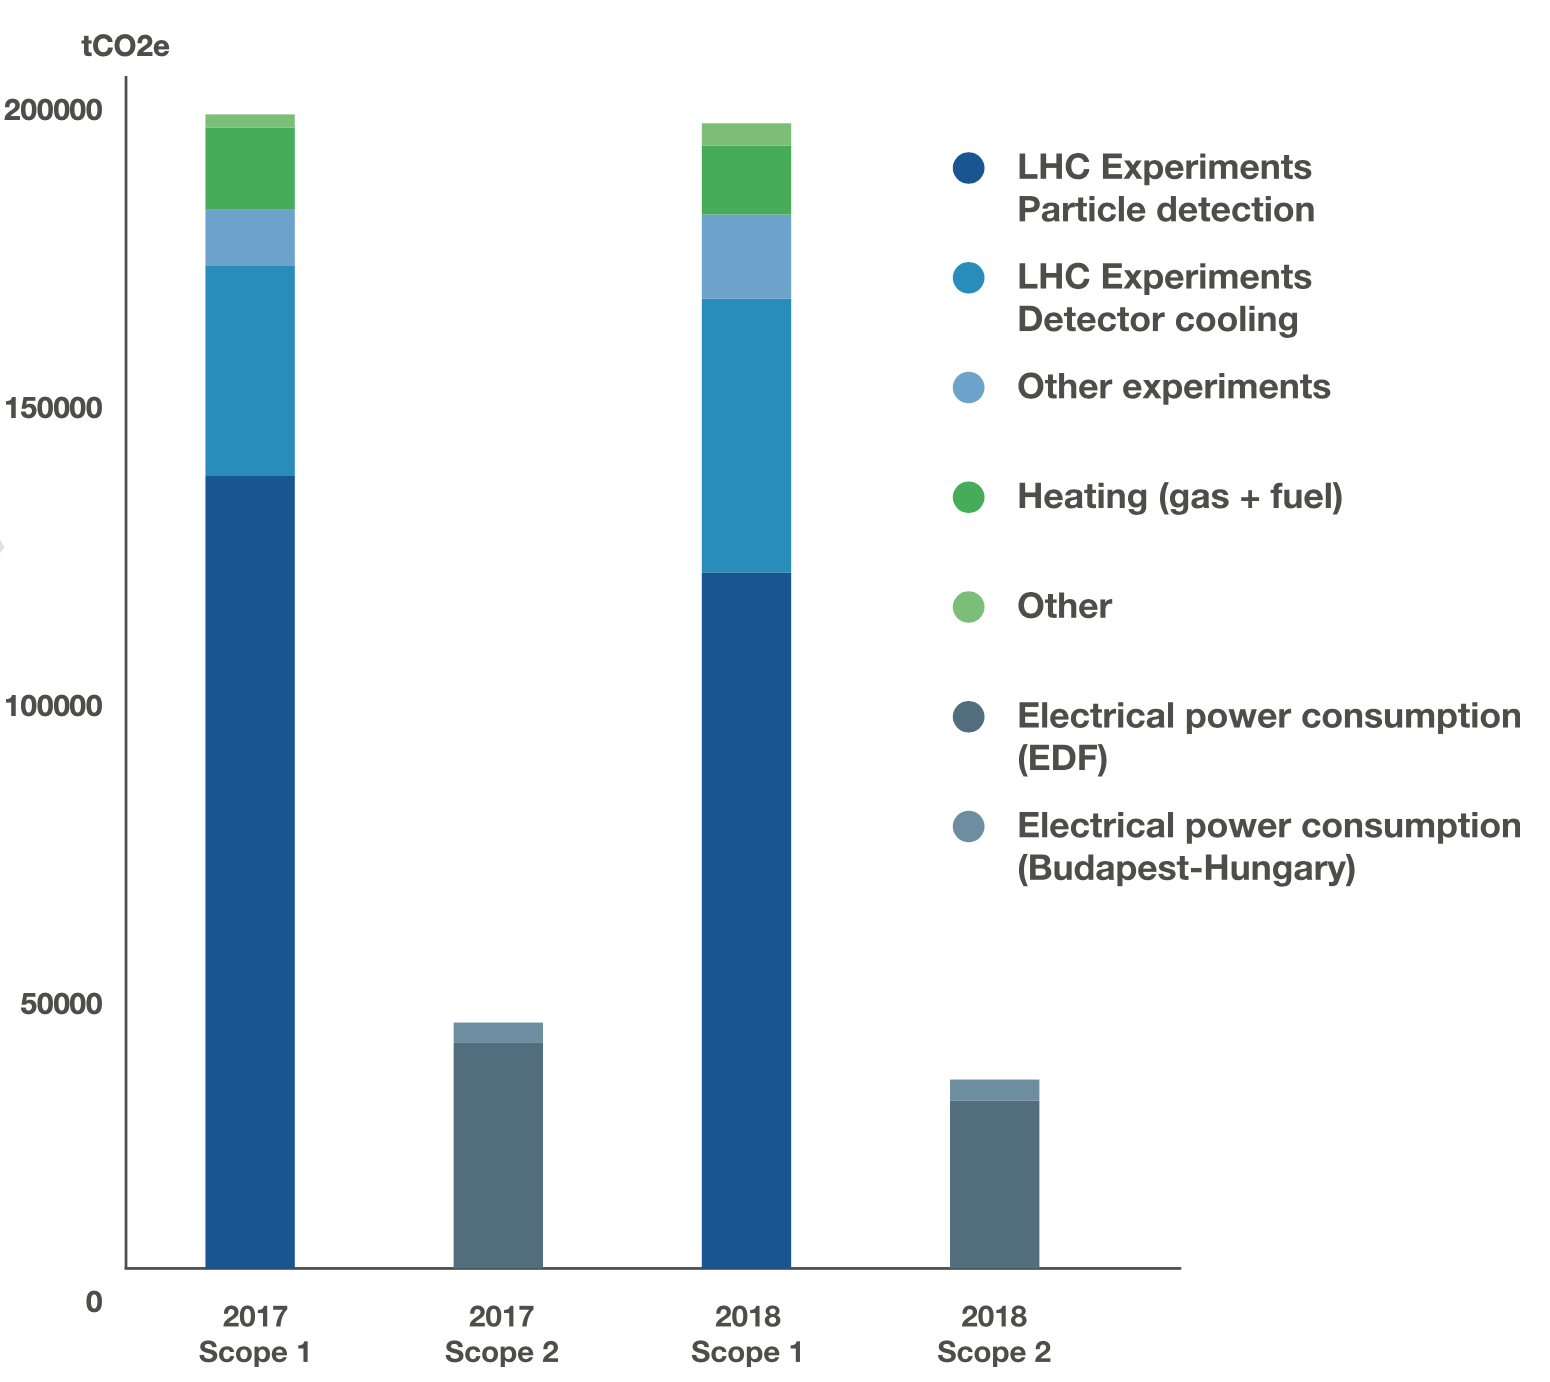
\includegraphics[width=.8\textwidth]{Technology/cern_co2.png}}
    \caption[CERN Scope 1 and Scope 2 emissions for 2017 and 2018]{CERN Scope 1 (direct) and Scope 2 (indirect, by electricity consumption) emissions for 2017 and 2018, in CO$_2$ equivalent tons, by category; ``other'' includes air conditioning, emergency generators and CERN vehicle fleet fuel consumption (reproduced from Ref.~\cite{envrep2020}).  `Budapest' refers to electricity use at the (now inactive) Wigner data centre in Hungary.}\label{fig:cern_co2}
\end{figure}

\begin{figure}
    \captionsetup{type=figure}
    {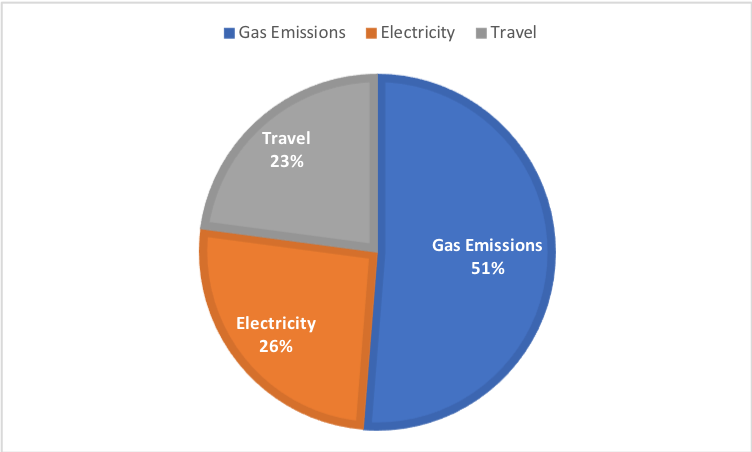
\includegraphics[width=.8\textwidth,trim=0.05cm 0.2cm 0.05cm 0.2cm , clip=true]{Technology/LHCbEmissionsCo2ePie.png}}
    \caption[Expected relative emissions from LHCb operations in Run 3]{Expected relative contribution to CO$_2$ equivalent emissions from LHCb operations in Run 3. The total emissions are estimated to be 4,400 tonnes CO$_2$ equivalent per annum.}\label{fig:lhcb_co2}
\end{figure}

\paragraph{Direct emissions}

Direct emissions from LHCb are dominated by losses of gases with sizeable global warming potential (GWP). The GWP is the heat absorbed by a GHG in the atmosphere as a multiple of the same mass of CO$_2$.  It thus allows conversion into CO$_2$ equivalent emissions. As some gases break down, they have time-dependent values, and we use the 100 year value~\cite{AR5}. The gases are utilised in LHCb in detector cooling systems and in the detection systems. Improvements made in the cooling systems of LHCb mean that emissions are now dominated by the detection system in Upgrade I. All systems are closed, with emissions being the result of losses.

In the original LHCb detector of Run 1 and 2, the gas C$_6$F$_{14}$ (GWP 7910) was used in cooling plants. For upgrade I, ``Novec 649" (GWP 1) is planned to be used, along with 
increased use of low-impact CO$_2$ based cooling.
For Upgrade II, lower operating temperatures are foreseen, and the GWP of the cooling systems will be considered.

In the detector systems, the Ring Imaging Cherenkov Systems (RICH1 and 2) and Muon systems of Upgrade I use GHGs. The RICH2 system currently uses CF$_4$ (GWP 6630) and RICH1 C$_4$F$_{10}$ (GWP 9200) radiators. R\&D will be pursued for Upgrade II on alternative gases, RICH2 is looking at CO$_2$ use, where a test has already been performed, and leakless systems. Significant effort has been made to minimise leaks.  
In the original LHCb detector, GEM detectors (gas electron multiplier detectors) were utilised in a part of the muon system. The removal of these for Upgrade I reduces the detector system emissions by 40\%. 
Recirculating systems are used throughout. The study of alternative gas mixture will be conducted to reduce the CF$_4$ consumption in the proposed future muon systems.

The CO$_2$ equivalent emissions expected in Run~3 are shown in \fref{fig:LHCbCO2e}. These are taken from the average values of annual usage during Run 2 for the detector systems that are still present, or that have been replaced with similar systems for Run~3. 

\begin{figure}
    \captionsetup{type=figure}
    {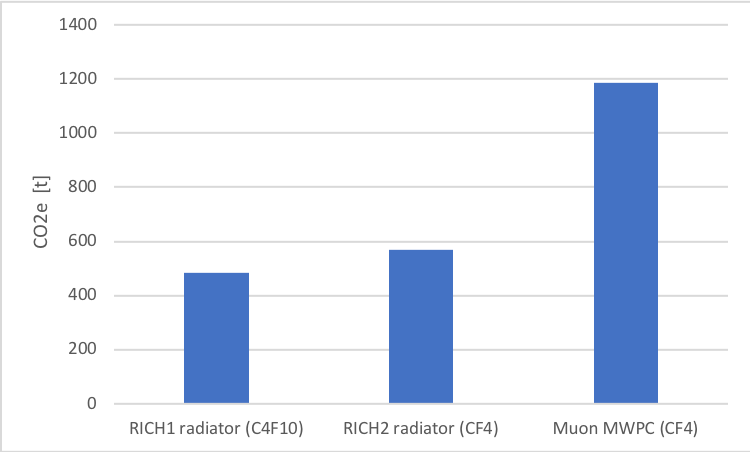
\includegraphics[width=.8\textwidth,trim=0.05cm 0.2cm 0.05cm 0.2cm , clip=true]{Technology/lhcb_co2e.png}}
    \caption[Expected Scope 1 emissions from LHCb detector gas systems in Run 3]{Expected Scope 1 (direct)  emissions in CO$_2$ equivalent tonnes from the LHCb detector gas systems in Run 3. The data is taken from the annual emissions of the systems, or predecessors, during Run 2.}\label{fig:LHCbCO2e}
\end{figure}

\paragraph{Power consumption}
\label{sec:powerconsumption}
CERN peak power demand, with the full accelerator chain running, is about $180$~MW, which brings the total annual energy consumption to $1.2$~TWh. This very large energy demand is partially mitigated by the fact that the electricity procurement is mainly from France, whose production capacity is 87.9$\%$ carbon-free (2017-figures). This keeps the contribution from the electrical power to the total CERN emission budget below 20$\%$, as shown in \fref{fig:cern_co2}.\footnote{It was argued in \sref{sec:Energy} that French energy production is part of the common EU~market and that it would therefore be more appropriate to use a conversion factor for an EU mix, which is about a factor of five higher than that for France~\cite{EUmix}.} Nevertheless, guided by the Energy Management Panel, EMP, CERN is spending a large effort to improve energy efficiency, with special focus on the accelerator sector. As an example, in the transition to the \acrshort{hl-lhc}, with a tenfold increase in luminosity, the Organization’s immediate priority is to limit the increase in energy consumption to 5$\%$ up to the end of 2024.
 
LHCb during a normal data taking period of Run 2 had a peak power demand stably around 5.5~MW, of which 4.6~MW was from the experiment dipole magnet, and the rest was from the detector electronics and the online computing farm.  The Run 3 expectation is for an increase of $\sim$1.5~MW due to the increased demand of data processing power, which is to be compared to the five-fold increase in luminosity.
For Run 5 and beyond, the contribution of online computing is expected to increase substantially, as a consequence of a further order of magnitude increase in the data throughput.

For the power dissipated by the LHCb magnet, an important mitigation has been implemented very recently by CERN with the installation of a heat-recovery plant at the experimental site. This is intended to use the
hot water produced by the magnet and the machine cooling systems to heat a new residential area in the
town of Ferney-Voltaire next to the LHCb site. Thanks to this project, up to 8000 people’s homes will be heated at a lower cost and with reduced CO$_2$ emissions, corresponding to $\sim$2.5\% of the total CERN emission budget per year. 

\paragraph{Digital technologies}
The power consumption of the online computing farm at LHCb has been about 530~kW on average during Run~2 of the LHC. To cope with the significantly increased computing needs after Upgrade~I, a new data centre has recently been installed at Point~8 and the power consumption for computing is going to increase to 2000~kW for the upcoming data taking periods. 
The new computing data centre at Point~8 is located in a surface building and for practical reasons could not be included in the heat recovery project discussed in Sec.~\ref{sec:powerconsumption} above. However, great care has been put into the design to optimise its power efficiency, for example by implementing a state-of-the-art indirect free air cooling system with adiabatic assist~\cite{lbldcreport}.
A \acrshort{pue} of better than 1.08 has been achieved for the new data centre at Point~8, a value that compares favourably with other large computing centres~\cite{pue-data}. 

While it does not seem feasible to further improve the PUE of the data centre, energy savings could potentially be achieved by adjusting the operating mode to the actual computing needs at a given point in time.  Significant improvements in energy efficiency can be achieved by rewriting software so that it can efficiently exploit today's highly parallel computing architectures. LHCb has been doing this in preparation for Run~3 data taking and the impact of these activities on the energy efficiency of our software has been documented in~\cite{hlt1-energy-eff}. In total the energy efficiency of HLT1 (High Level Trigger 1) software has been improved by a factor $4.8\times$ on \acrshort{cpu}s, with the improvements coming in roughly equal parts from physics optimizations and the rewrite of the underlying software framework. A further improvement in energy efficiency  can also be achieved by porting suitable algorithms from CPUs to more efficient technologies such as \acrshort{gpu}s, field programmable gate arrays (FPGAs) or even custom-made application specific integration circuits (ASICs). LHCb has demonstrated this with the Allen project~\cite{Allen}, which implemented HLT1 on GPUs, leading to an overall improvement in energy efficiency of up to $19$ times compared to the Run~2 architecture. These improvements require significant effort and investment, above all in the training and retention of scientists able to effectively program across a range of modern computing architectures. 

The energy efficiency of the underlying computer hardware has also improved substantially over time. For example, the
AMD~7502~\cite{AMD7502} CPUs, which were evaluated as candidates for LHCb's Run~3 HLT, are $2.6$ times more energy efficient than 
the benchmark E5-2630~Xeon CPUs used by LHCb during Run~2. 
Within a given computing architecture, energy savings can also be achieved by purchasing more expensive, higher quality hardware. 
As an example from the world of CPU, the more expensive AMD~7742~\cite{AMD7742}
provides twice the number of CPU cores and threads as the cheaper AMD~7502~\cite{AMD7502},
while its specified power consumption is only 25\% higher. The energy consumption and carbon footprint from data transfer, data storage and offline computing are much harder to assess than those for online computing, due to the distributed nature of the computing model with data centres and users distributed over many different countries. The GRAND collaboration has performed pioneering work in this direction~\cite{GRAND}.

\paragraph{Mobility}
As an international collaboration operating in an international field of research, travel is an intrinsic part of how LHCb operates. We have estimated the environmental impact of travel in order to attend LHCb collaboration meetings and international conferences. We have not taken into account local commuter travel or travel related to on-site work at LHCb, such as shifts, although the latter is probably significant.

The impact of travel per participant for a typical LHCb collaboration week, pre-pandemic, corresponded to around 0.5 \acrshort{tco2e} with the average LHCb week in 2019 leading to travel-emissions of $\sim$ 180$\,\mathrm{tCO_2e}$. The Speakers' Bureau database provides a complete record of all LHCb conference talks, allowing us to estimate the environmental impact in terms of $\mathrm{tCO_2e}$ per year. LHCb weeks and conference travel contribute a total of approximately $1,000\,\mathrm{tCO_2e}$ per annum, a similar carbon footprint to the Run~3 experiment's projected electricity use due to online computing and the magnet (French energy mix). LHCb weeks contribute about three times as much to  LHCb's carbon footprint as conference travel.
 The carbon footprint of virtual conference attendance is calculated according to the life cycle and operating costs of endpoint devices estimates in Ref.~\cite{VideoConCO2}, and is small.

LHCb, in common with other High Energy Physics collaborations, had extensive experience with virtual meetings before COVID, and videoconferencing
technology has already helped to reduce travel-related emissions over the past decade.
However, the pandemic, as well as recent improvements to the videoconferencing software infrastructure, have shown us ways 
in which the organisation of virtual meetings can be improved and made more inclusive. 
At the same time the pandemic has also reminded us of the ongoing importance of in-person interaction,
not least to avoid fracturing the collaboration between those who can regularly travel to CERN in eco-friendly ways and those who cannot.
The collaboration has only just started to navigate this tension but is actively exploring ways to reduce its 
travel-related environmental impact.

\end{casestudy}

\end{document}




